\newpage
\section{Nền tảng toán học}

\paragraph{}{Các kiến thức trong phần này được trích dẫn từ sách Giáo trình bài tập Xác suất thống kê \cite{xstk}, trường Đại học Khoa học tự nhiên, ĐHQG-HCM và một số trang thông tin khác.}

\subsection{Chuẩn hóa Z-score}
\label{label:standart scaler}

\paragraph{}{\textbf{Chuẩn hóa Z-score} là phương pháp biến đổi dữ liệu có phân phối chuẩn bất kì về phân phối chuẩn hóa.} Tức là, nếu \(u\) là giá trị chuẩn hóa của dữ liệu ban đầu thì \textbf{\(u \sim N(0,1)\)}.

\paragraph{}{Dữ liệu sau quá trình chuẩn hóa thường được gọi là dữ liệu chuẩn hóa hoặc \textbf{điểm Z (Z-scores)}. Giá trị của Z-score thường nằm trong khoảng \([-3, 3]\).}

\paragraph{}{\textbf{Công thức chuẩn hóa đối với tổng thể:} Nếu một biến ngẫu nhiên $X$ tuân theo phân phối chuẩn (tức là $X \sim N(\mu, \sigma^2)$), thì điểm Z được tính bằng công thức:}
\[
Z = \frac{X - \mu}{\sigma}
\]
\paragraph{}{Trong đó:}
\begin{itemize}
    \item $Z$: Điểm Z chuẩn hóa.
    \item $X$: Giá trị của biến ngẫu nhiên hoặc một giá trị cụ thể từ tổng thể.
    \item $\mu$: Trung bình của tổng thể.
    \item $\sigma$: Độ lệch chuẩn của tổng thể.
\end{itemize}

\paragraph{}{\textbf{Công thức chuẩn hóa đối với dữ liệu mẫu:}}

\paragraph{}{Trong thực tế, chúng ta thường làm việc với dữ liệu mẫu và không biết $\mu$ và $\sigma$. Khi đó, chúng ta sẽ ước lượng chúng bằng trung bình mẫu ($\bar{x}$) và độ lệch chuẩn mẫu ($s$). Điểm Z cho một giá trị cụ thể $x$ trong mẫu được tính bằng công thức:}
\[
z = \frac{x - \bar{x}}{s}
\]
\paragraph{}{Trong đó:}
\begin{itemize}
    \item $z$: Giá trị chuẩn hóa (điểm Z) của $x$ dựa trên mẫu.
    \item $x$: Giá trị dữ liệu gốc trong mẫu.
    \item $\bar{x}$: Trung bình mẫu của  dữ liệu (sample mean).
    \item $s$: Độ lệch chuẩn mẫu của dữ liệu.
\end{itemize}



\subsection{Hiệp phương sai (Covariance)}

\paragraph{}{\textbf{Hiệp phương sai} (Covariance) \cite{thongke-descriptive-statistics} là thước đo mối liên hệ tuyến tính giữa hai biến ngẫu nhiên $X$ và $Y$. Ký hiệu: $cov(X, Y)$. Hiệp phương sai giữa hai biến ngẫu nhiên $X$ và $Y$ còn được định nghĩa là kỳ vọng của tích giữa độ lệch của $X$ và $Y$ so với giá trị kỳ vọng của chúng.}

\paragraph{}{\textbf{Công thức tính hiệp phương sai:}}

\begin{center}
\large $cov(X, Y) = E[(X-E(X))(Y-E(Y))]$
\end{center}

Công thức tính trên tổng thể:
\begin{center}
\large $cov(X,Y) = \frac{1}{N} \sum_{i=1}^{N} (x_i - \mu_X)(y_i - \mu_Y)$
\end{center}

Công thức tính trên mẫu:
\begin{center}
\large $cov(X,Y) = \frac{1}{n-1} \sum_{i=1}^{n} (x_i - \bar{x})(y_i - \bar{y})$
\end{center}

Trong đó:
\begin{itemize}
    \item \( x_i, y_i \) là giá trị của quan sát thứ \(i\).
    \item \( \mu_X, \mu_Y \) là giá trị trung bình của tổng thể.
    \item \( \bar{x}, \bar{y} \) là giá trị trung bình của mẫu.
    \item \( N \) là tổng số quan sát của tổng thể.
    \item \( n \) là tổng số quan sát của mẫu.
\end{itemize}
\paragraph{}{\textbf{Trực quan bằng đồ thị:}}
\begin{figure}[H]
    \centering
    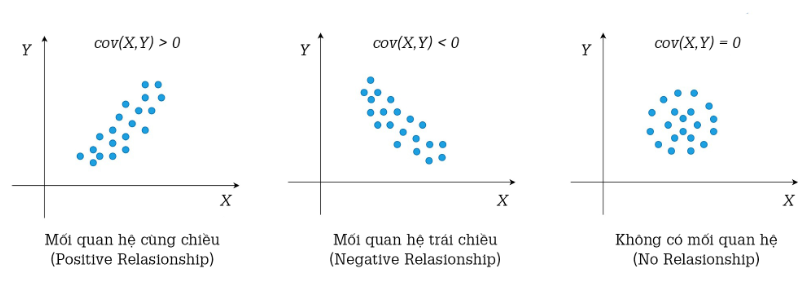
\includegraphics[width=\textwidth]{img/corvariance.png}
    \caption{Minh họa hiệp phương sai giữa hai biến ngẫu nhiên $X$ và $Y$.}
    \label{fig:covariance}
\end{figure}

\paragraph{}{Đồ thị trên minh họa ba trường hợp có thể xảy ra khi tính hiệp phương sai:}

\begin{itemize}
    \item Khi \(\text{cov}(X,Y) > 0\): Hai biến \(X\) và \(Y\) có quan hệ tuyến tính thuận, khi \(X\) tăng thì \(Y\) cũng tăng.
    \item Khi \(\text{cov}(X,Y) < 0\): Hai biến \(X\) và \(Y\) có quan hệ tuyến tính nghịch, khi \(X\) tăng thì \(Y\) giảm và ngược lại.
    \item Khi \(\text{cov}(X,Y) = 0\): Hai biến \(X\) và \(Y\) không có mối quan hệ tuyến tính với nhau.
\end{itemize}
\subsection{Ma trận hiệp phương sai (Covariance matrix)}

\paragraph{}{\textbf{Ma trận hiệp phương sai} là một ma trận vuông chứa các hiệp phương sai giữa các biến trong một tập dữ liệu. Nếu một tập dữ liệu có \( p \) biến ngẫu nhiên \( X_1, X_2, \dots, X_p \), thì ma trận hiệp phương sai \( \Sigma \) có dạng:}

\[
\Sigma =
\begin{bmatrix}
\text{Var}(X_1) & \text{Cov}(X_1, X_2) & \dots & \text{Cov}(X_1, X_p) \\
\text{Cov}(X_2, X_1) & \text{Var}(X_2) & \dots & \text{Cov}(X_2, X_p) \\
\vdots & \vdots & \ddots & \vdots \\
\text{Cov}(X_p, X_1) & \text{Cov}(X_p, X_2) & \dots & \text{Var}(X_p)
\end{bmatrix}
\]

Trong đó:
\begin{itemize}
\item \( \text{Var}(X_i) = \text{Cov}(X_i, X_i) \) là phương sai của biến \( X_i \).
\item \( \text{Cov}(X_i, X_j) \) là hiệp phương sai giữa hai biến \( X_i \) và \( X_j \).
\end{itemize}
\paragraph{}{\textbf{Công thức tổng quát:}
Giả sử có một tập dữ liệu với \( n \) quan sát và \( p \) biến ngẫu nhiên được biểu diễn dưới dạng ma trận \( X \) có kích thước \( n \times p \), với mỗi hàng là một quan sát và mỗi cột là một biến. Khi đó, ma trận hiệp phương sai được tính bằng công thức:}

\[
\Sigma = \frac{1}{n - 1} \sum_{i=1}^{n} (X_i - \bar{X})(X_i - \bar{X})^T
\]

Trong đó:
\begin{itemize}
\item \( X_i \) là vector giá trị của các biến tại quan sát thứ \( i \).
\item\( \bar{X} \) là vector trung bình của từng biến.
\end{itemize}
\paragraph{}{\textbf{Tính chất:}}
\begin{itemize}
    \item Ma trận hiệp phương sai là \textbf{ma trận đối xứng}.
    \item Đường chéo chứa phương sai của từng biến.
    \item Nếu các biến không có tương quan (độc lập tuyến tính), thì các phần tử ngoài đường chéo bằng 0.
\end{itemize}

\pagebreak
